\documentclass[a4paper, 14pt]{extarticle}

\usepackage{../generalPreamble}
\usepackage{../reportFormat}
\usepackage{../sourceCode}

\begin{document}
\begin{titlepage}
    \centering
    {\bfseries
        \uppercase{
            Минобрнауки России \\
            Санкт-Петербургский государственный \\
            Электротехнический университет \\
            \enquote{ЛЭТИ} им. В.И.Ульянова (Ленина)\\
        }
        Кафедра ИБ

        \vspace{\fill}
        \uppercase{Отчёт} \\
        по лабораторной работе №8 \\
        по дисциплине \enquote{Криптография и защита информации} \\
        Тема: Изучение цифровой подписи
    }

    \vspace{\fill}
    \begin{tabularx}{0.8\textwidth}{l X c r}
        Студент гр. 6304 & & \underline{\hspace{3cm}} & Корытов П.В.\\
        Преподаватель & & \underline{\hspace{3cm}} & Племянников А.К.
    \end{tabularx}

    \vspace{1cm}
    Санкт-Петербург \\
    \the\year{}
\end{titlepage}
\section*{Цель работы}
Исследовать алгоритмы создания и проверки цифровой подписи, алгоритмы генерации ключевых пар RSA, DSA, ECDSA и получить практические навыки работы с ними, в том числе и в программном продукте CrypTool 1.

\section{Генераторы ключевых пар}
\subsection{Основные теоретические положения}
\subsubsection{RSA}
\begin{enumerate}
    \item Генерация двух больших простых чисел $p, q$
    \item Вычисление $n = p \cdot q$
    \item Выбор $e < n$, взаимно простого с $\varphi(n)$
    \item Вычисление $d : e \cdot d = 1 \bmod \varphi(n)$
    \item $(e, n)$ --- открытый ключ, $d$ --- закрытый ключ, $p, q$ --- уничтожаются
\end{enumerate}

\subsubsection{DSA}
\begin{enumerate}
    \item Выбирается $p$ длиной $[512, 1024]$ бит с числом битов, кратным $64$.
    \item Выбирается число $q$ с тем же размером дайджеста $160$ бит, такое, что $(p - 1) = 0 \bmod q$
    \item Выбирается $e_1 : e_1^q = 1 \bmod p$
    \item Выбирается $d \in \mathbb{Z}: d < q$, вычисляется $e_2 = e_1^d \bmod p$
    \item $(e_1, e_2, p, q)$ --- открытый ключ, $d$ --- закрытый ключ
\end{enumerate}

\subsubsection{ECDSA}
\begin{enumerate}
    \item Выбирается эллиптическая кривая $E_p(a,b)$, $p$ --- простое число
    \item Выбирается $q$ --- простое число --- порядок одной из циклических подкргупп группы точек эллиптической кривой: $q \times (x_0, y_0) = 0$
    \item Выбирается закрытый ключ --- $d$
    \item Выбирается точка на кривой $e_1 = (x_1, y_1)$
    \item Выбирается точка на кривой $e_2 = d \times e_1$
    \item Открытый ключ --- $(a, b, q, p, e_1, e_2)$
\end{enumerate}

\subsection{Формулировка задания}
\begin{enumerate}
    \item Перейти к утилите «Digital Signatures/PKI->PKI/Generate…».
    \item Сгенерировать ключевые пары по алгоритмам RSA-2048, DSA-2048, EC-239. Зафиксируйте время генерации в таблице.
    \item С помощью утилиты «Digital Signatures/PKI-> PKI/Display…» вывести сгенерированный открытый ключ и сохранить соответствующий скриншот.
\end{enumerate}

\subsection{Ход работы}
\begin{enumerate}
    \item Открыта утилита генерации ключей.
        \begin{figure}[h]
            \centering
            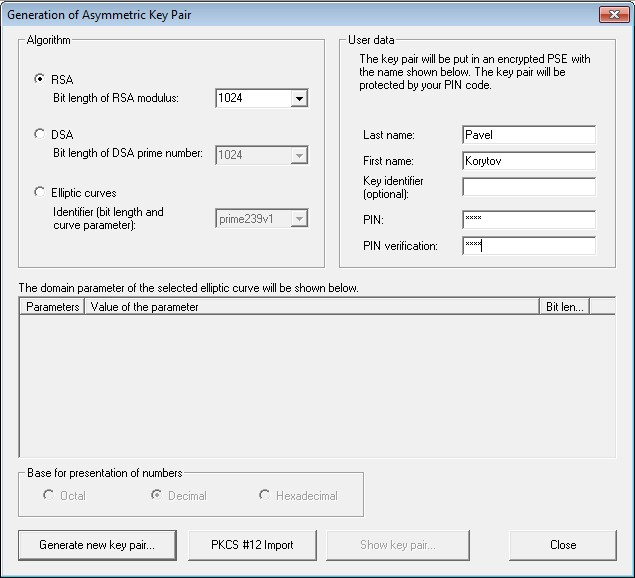
\includegraphics[width=\textwidth]{img/S001.jpg}
            \caption{Интерфейс утилиты генерации ключей}%
            \label{img:1:1}
        \end{figure}
    \item Измерено время генерации ключевых пар.
        \begin{table}[h]
            \centering
            \begin{tabular}{@{}ll@{}}
                \toprule
                \textbf{Алгоритм} & \textbf{Время создания ключа} (с.) \\ \midrule
                RSA-2048 & 2.938                     \\
                DSA-2048 & 9.343                     \\
                EC-239   & 0.014                     \\ \bottomrule
            \end{tabular}
        \end{table}
        \FloatBarrier{}
    \item Полученные сертификаты:
        \lstinputlisting[style=framed_num,caption=сертификат с DSA-2048]{./key/dsa.key}
        \begin{figure}[h]
            \centering
            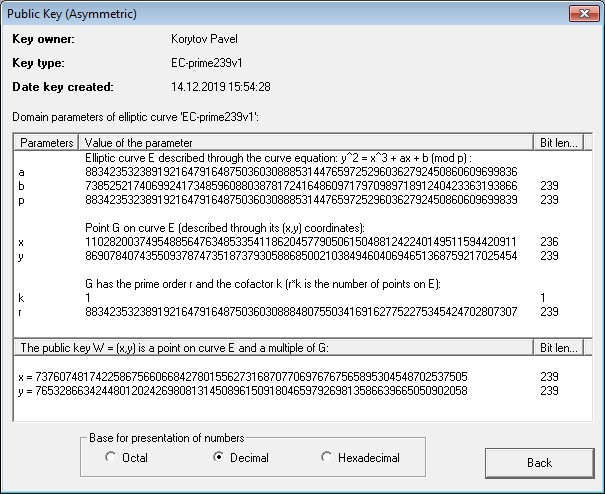
\includegraphics[width=\textwidth]{img/S002.jpg}
            \caption{Публичные парамеры ключа с EC-239}%
            \label{img:1:2}
        \end{figure}
        \FloatBarrier{}

        \lstinputlisting[style=framed_num,caption=сертификат с RSA-2048]{./key/rsa.key}

\end{enumerate}

\section{Процессы создания и проверки цифровой подписи}
\subsection{Основые теоретические положения}
\begin{figure}[h]
    \centering
    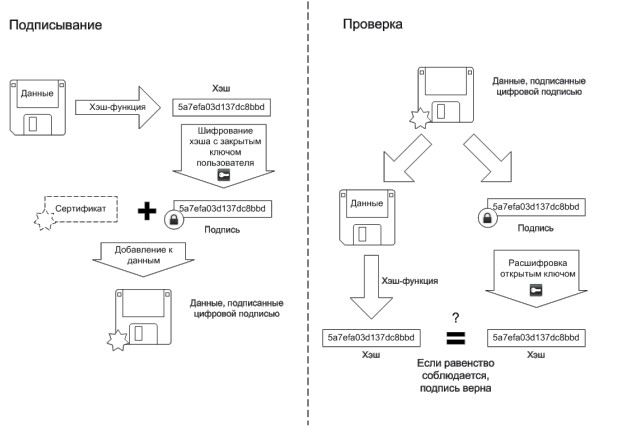
\includegraphics[width=\textwidth]{img/S003.jpg}
    \caption{Обобщенная схема подписывания и проверки цифровой подписи}%
    \label{img:2:1}
\end{figure}
\FloatBarrier{}

\subsection{Формулировка задания}
\begin{enumerate}
    \item Открыть текст не менее 5000 знаков. Перейти к приложению Digital Signatures/PKI-> Sign Document…
    \item Задайте хэш-функцию, и другие параметры цифровой подписи.
    \item Создайте подпись ключами, сгенерированными в предыдущем задании. Зафиксируйте время создания цифровой подписи для каждого ключа.
    \item Сохраните скриншот цифровой подписи с помощью приложения Digital Signatures/PKI-> Extract Signature.
    \item Выполните процедуру проверки подписи Digital Signatures/PKI-> Verify Signature для случаев сохранения и нарушения целостности исходного текста. Сохраните скриншоты результатов.
\end{enumerate}

\subsection{Ход работы}
\begin{enumerate}
    \item Создан текст, удовлетворяющий требованиям.
        \begin{figure}[h]
            \centering
            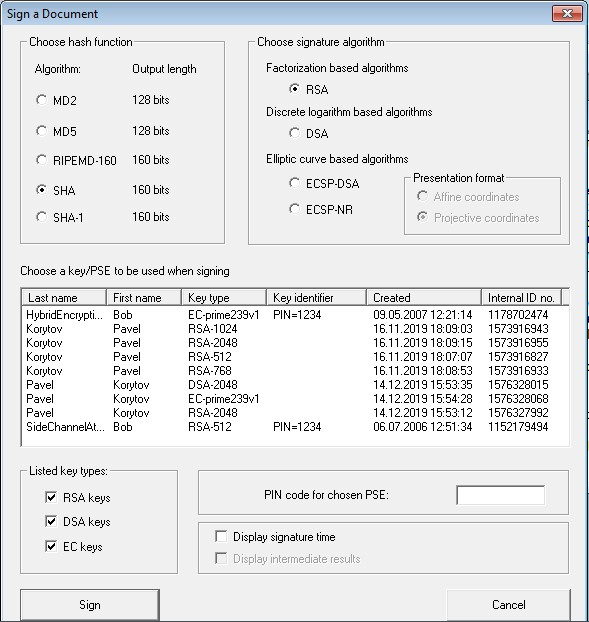
\includegraphics[width=0.8\textwidth]{img/S004.jpg}
            \caption{Утилита подписания документа}%
            \label{img:2:2}
        \end{figure}
        \FloatBarrier{}
    \item Измерено время подписания всеми созданными ключами.
        \begin{table}[h]
            \centering
            \begin{tabular}{@{}ll@{}}
                \toprule
                \textbf{Алгоритм} & \textbf{Время подписания (с.)} \\ \midrule
                RSA-2048          & 0.016                          \\
                DSA               & 0.000                          \\
                EC-239            & 0.031                          \\ \bottomrule
            \end{tabular}
        \end{table}
        \FloatBarrier{}
    \item Извлечены сигнатуры подписей:
        \lstinputlisting[style=framed_num,caption=сигнатура RSA-2048]{./key/rsa_sign.hex}
        \lstinputlisting[style=framed_num,caption=сигнатура DSA-2048]{./key/dsa_sign.hex}
        \lstinputlisting[style=framed_num,caption=сигнатура EC-239]{./key/ec_sign.hex}
    \item Выполнена проверка подписей.
        \begin{figure}[h]
            \centering
            \begin{subfigure}[b]{0.42\textwidth}
                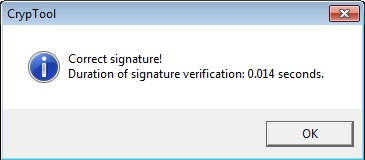
\includegraphics[width=\textwidth]{img/S005.jpg}
                \caption{Успешная валидация}
            \end{subfigure}%
            \hspace{1cm}
            \begin{subfigure}[b]{0.42\textwidth}
                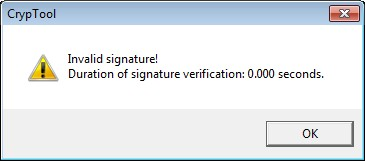
\includegraphics[width=\textwidth]{img/S006.jpg}
                \caption{Ошибка валидации}
            \end{subfigure}
            \caption{Валидация подписей}
        \end{figure}
        \FloatBarrier{}

        \begin{table}[h]
            \centering
            \begin{tabular}{@{}lll@{}}
                \toprule
                \textbf{Алгоритм} & \textbf{Время упешной проверки (с.)} & \textbf{Время неудачной проверки (с.)} \\ \midrule
                RSA-2048          & 0.000                                & 0.000                                  \\
                DSA               & 0.014                                & 0.000                                  \\
                EC-239            & 0.000                                & 0.000                                  \\ \bottomrule
            \end{tabular}
        \end{table}

\end{enumerate}

\section{Схемы цифровой подписи на эллиптических кривых}
\subsection{Основые теоретические положения}
\begin{figure}[h]
    \centering
    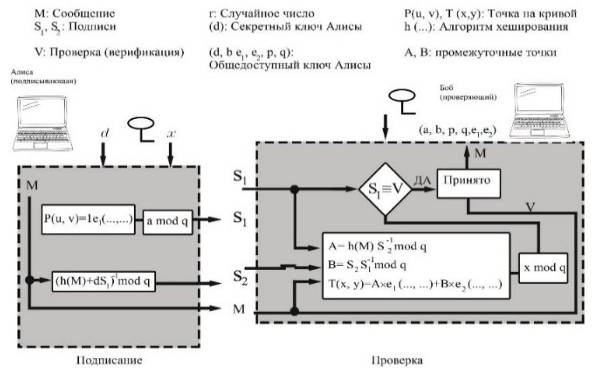
\includegraphics[width=\textwidth]{img/S008.jpg}
    \caption{Схема цифровой подписи ECDSA}%
    \label{img:3:1}
\end{figure}
$d$ --- закрытый ключ, $(a, b, q, p, e_1, e_2)$ --- открытый ключ.

Алгоритм подписания:
\begin{enumerate}
    \item Выбирается секретное случайное число $r: r \in (1, q - 1)$
    \item Выбирается третья точка на кривой: $P(u, v) = r \times e_1$
    \item Вычисляется первая часть подписи по формуле:
    \begin{equation*}
        S_1 = u \bmod q,
    \end{equation*}
    где $q$ --- абсцисса.
    \item Вычисляется вторая часть подписи по формуле:
    \begin{equation*}
        S_2 = (h(M) + d \times S_1) \times r^{-1} \bmod q,
    \end{equation*}
    где $h(M)$ --- дайджест сообщения, $d$ --- закрытый ключ\\
\end{enumerate}

Алгоритм проверки:
\begin{enumerate}
    \item Вычисляются промежуточные результаты:
    \begin{equation*}
        A = h(M) \times S_2^{-1} \bmod q
    \end{equation*}
    \begin{equation*}
        B = S_2^{-1} \times S_1 \bmod q
    \end{equation*}
    \item Восстанавливаем третью точку:
    \begin{equation*}
        T(x,y) = A \times e_1 + B \times e_2
    \end{equation*}
    \item Верификатор $V = x \bmod q$ сравнивается с $S_1$
\end{enumerate}

\subsection{Формулировка задания}
\begin{enumerate}
    \item Выполните процедуру создание подписи «Digital Signatures/PKI-> Sign Document…» алгоритмом ECSP-DSA в пошаговом режиме (Display inter.results=ON). Зафиксируйте скриншоты последовательности шагов.
    \item Выполните процедуру проверки подписи ECSP-DSA для случаев сохранения и нарушения целостности исходного текста. Сохраните скриншоты результатов.
    \item Проверить лекционный материал по ECDSA, выполнив создание и проверку подписи сообщения M (принять $M=h(M)$) приложением Indiv.Procedures->Number Theory->Point Addition on EC.\@
\end{enumerate}

\subsection{Ход работы}
\begin{enumerate}
    \item Выполнено создание подписи алгоритмом ECSP-DSA.\@
        \lstinputlisting[style=framed_num,caption=Лог подписания ECSP]{./key/escp_dsa.log}
    \item Выполнена проверка подписей.
        \begin{figure}[h]
            \centering
            \begin{subfigure}[b]{0.42\textwidth}
                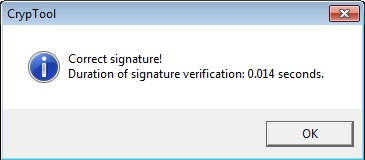
\includegraphics[width=\textwidth]{img/S005.jpg}
                \caption{Успешная валидация}
            \end{subfigure}%
            \hspace{1cm}
            \begin{subfigure}[b]{0.42\textwidth}
                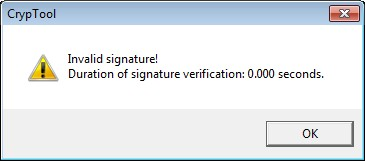
\includegraphics[width=\textwidth]{img/S006.jpg}
                \caption{Ошибка валидации}
            \end{subfigure}
            \caption{Валидация подписей}
        \end{figure}
        \FloatBarrier{}

    \item Проведена проверка лекционного материала.
    \begin{figure}[h]
        \centering
        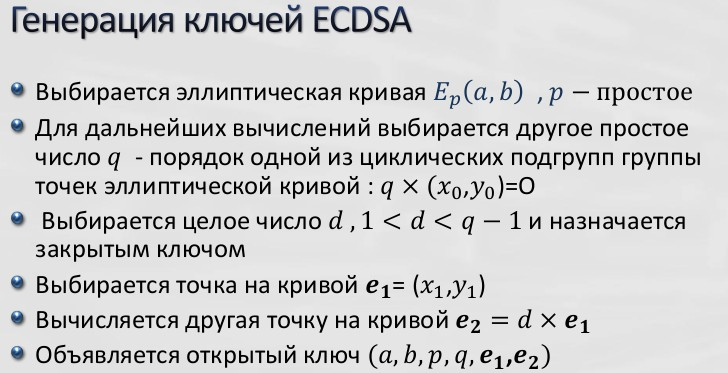
\includegraphics[width=\textwidth]{img/S009.jpg}
        \caption{Слайд с описанием генерации ключей ECDSA}%
        \label{img:3:2}
    \end{figure}
    \begin{figure}[h]
        \centering
        \begin{subfigure}[b]{0.49\textwidth}
        	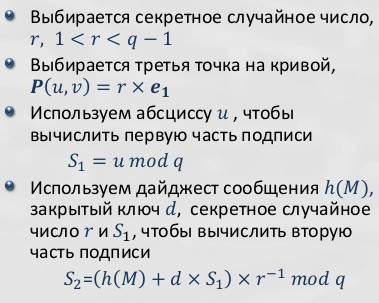
\includegraphics[width=\textwidth]{img/S011.jpg}
        	\caption{ECDSA подписание}
        \end{subfigure}%
        \hspace{6pt}
        \begin{subfigure}[b]{0.45\textwidth}
        	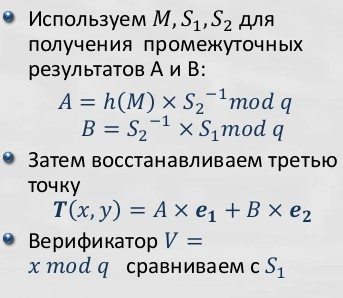
\includegraphics[width=\textwidth]{img/S012.jpg}
        	\caption{ECDSA проверка}
        \end{subfigure}
        \caption{Подписание и проверка}
    \end{figure}

    \begin{figure}[h]
        \centering
        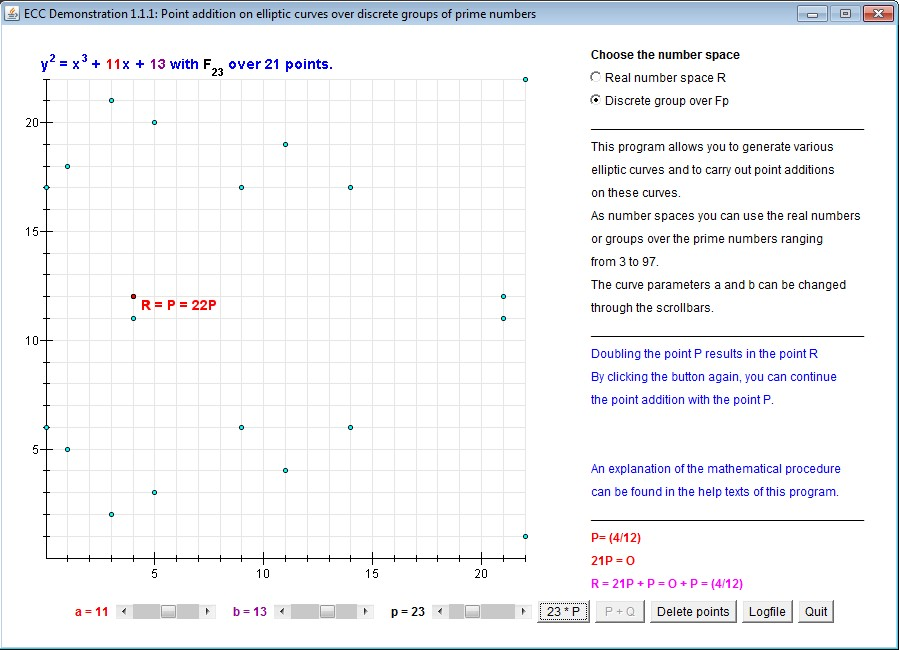
\includegraphics[width=0.8\textwidth]{img/S010.jpg}
        \caption{Утилита для вычислений на эллиптических кривых}%
        \label{img:3:3}
    \end{figure}
    \FloatBarrier{}

    Генерация ключей:
    \begin{itemize}
        \item Выбрана эллиптическая кривая $y^2 = x^3 + 11x + 13$ над $F_{23}$.\\
            $a = 11, b = 13, p = 23$
        \item $P:=(4, 12)$
        \item Путем перебора: $21 \times (4, 12) = O \Rightarrow q = 21$
        \item $d:= 10$ --- закрытый ключ
        \item $e_1 := (14, 17)$
        \item $e_2 = d \times e_1 = 10 \times (14, 17) = (5, 3)$
        \item Открытый ключ --- $(11, 13, 23, 21, (14, 17), (5, 3))$\\
    \end{itemize}

    Подписание:
    \begin{itemize}
        \item $r:= 13$
        \item $(u, v) = 13 \times (14, 17) = (14, 6)$
        \item $S_1 = u \bmod q = 14 \bmod 21 = 14$
        \item $M:=99, h(M) := M$.\\
            \begin{equation*}
                \begin{split}
                    S_2 &= (h(M) + d \times S_1) \times r^{-1} \bmod q \\
                    &= (99 + 10 \times 14) \times 13^{-1} \bmod 21 = 20
                \end{split}
            \end{equation*}
    \end{itemize}

    Проверка:
    \begin{itemize}
        \item $A = h(M) \times S_2^{-1} \bmod q = 99 \times 20^{-1} \bmod 21 = 6$
        \item $B = S_2^{-1} \times S_1 \bmod 21 = 7$
        \item $(x, y) = A \times e_1 + B \times e_2 = (14, 6) + O = (14, 6)$
        \item $x = S_1$ --- проверка пройдена.
    \end{itemize}


\end{enumerate}

\section{Демострация процесса подписи в среде PKI}
\subsection{Формулировка задания}
\begin{enumerate}
    \item Запустить демонстрационную утилиту «Digital Signatures/PKI-> Signature Demonstration…».
    \item Получите сертификат на ранее сгенерированную ключевую пару RSA-2048.
    \item Выполните и сохраните скриншоты всех этапов создания цифровой подписи документа.
    \item Сохраните скриншот сертификата для проверки этой цифровой подписи
\end{enumerate}

\subsection{Ход работы}
\begin{enumerate}
    \item Запущена указанная утилита.
    \begin{figure}[h]
        \centering
        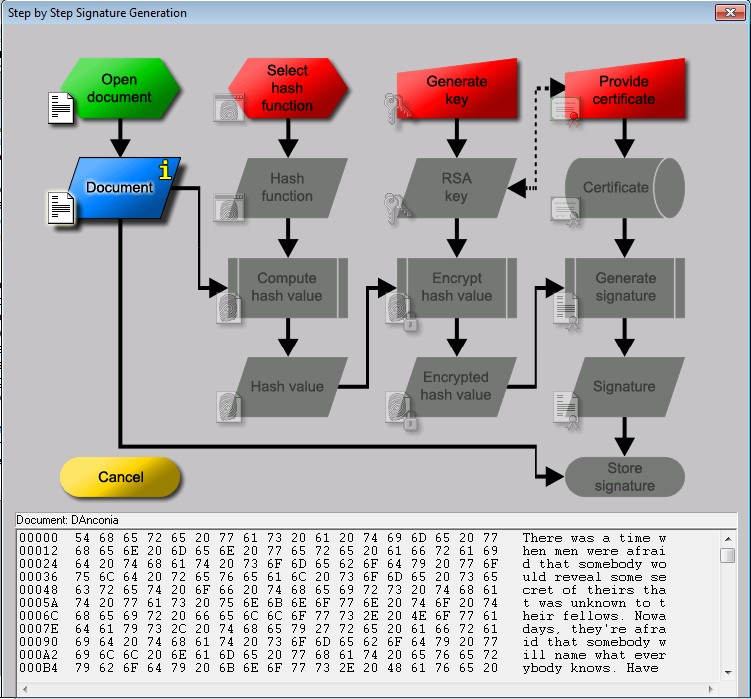
\includegraphics[width=0.7\textwidth]{img/S013.jpg}
        \caption{Вид Signature Demonstration}%
        \label{img:4:1}
    \end{figure}
    \FloatBarrier{}
    \begin{enumerate}
        \item Выбрана хэш-функция SHA-1
        \begin{lstlisting}[style=framed_num,caption=хэш-функция]
Name:                   SHA-1 
Length in bits:         160
Algorithm ID:           30 21 30 09 06 05 2B 0E 03 02 1A 05 00 04 14
        \end{lstlisting}
        \item Вычислен SHA-1 хэш текста
        \begin{lstlisting}[style=framed_num,caption=хэш текста]
B3 75 2B DA 2C EC 38 6A AE BD 4A A2 B7 78 B1 3D 8C 3C 9D B8
        \end{lstlisting}

        \item Сгенерирован RSA-ключ
        \begin{lstlisting}[style=framed_num,caption=ключ]
Bit length of N:         304
RSA modulus N:          5 153 404 714 761 008 744 896 344 126 074 269 264 270 224 690 453 913 630 460 946 340 383 627 809 721 221 384 320 487 569
phi(N) = (p-1)(q-1):    5 153 404 714 761 008 744 896 344 126 074 269 264 270 224 685 849 812 918 367 971 768 861 525 030 822 887 495 081 938 944
Public key:             65537
Private key:            2 239 403 892 025 554 542 409 676 737 819 386 215 071 665 300 949 338 878 834 879 045 507 230 592 685 124 631 466 782 721
        \end{lstlisting}
        \item Хэш зашифрован созданным ключом
        \begin{lstlisting}[style=framed_num,caption=шифрование текста]
Padding string:         01 00
Algorithm ID:           30 21 30 09 06 05 2B 0E 03 02 1A 05 00 04 14
Hash value:             B3 75 2B DA 2C EC 38 6A AE BD 4A A2 B7 78 B1 3D 8C 3C 9D B8

ASN-1 hash value:       01 00 30 21 30 09 06 05 2B 0E 03 02 1A 05 00 04 14 B3 75 2B DA 2C EC 38 6A AE BD 4A A2 B7 78 B1 3D 8C 3C 9D B8
Length in bits:         296

Encrypted hash value:   20 BA E4 EF B1 1F 42 67 38 1B B6 49 D1 09 73 4D F1 AF F3 54 FB C4 34 52 BC 92 A0 AB 1E 82 6C 62 8F A6 AA F6 5A 8B
Length in bits:         304
        \end{lstlisting}
        \item Создан сертификат для созданной ключевой пары
        \begin{lstlisting}[style=framed_num,caption=созданный сертификат]
Version:                  2 (X.509v3-1996)
SubjectName:              CN=Korytov Pavel [1576340635], DC=cryptool, DC=org
IssuerName:               CN=CrypTool CA 2, DC=cryptool, DC=org
SerialNumber:             C1:C5:9D:B5:B0:ED:58:C8
Validity  -  NotBefore:   Sat Dec 14 19:23:59 2019 (191214162359Z)
              NotAfter:   Mon Dec 14 19:23:59 2020 (201214162359Z)
Public Key Fingerprint:   E597 C0CC BD38 A551 F1C0 57A8 29AA 5A47 
SubjectKey:               Algorithm rsa (OID 2.5.8.1.1), Keysize = 512
              Public modulus (no. of bits = 302):
                0  287A48C1 4EAE7ABC  9CE3B671 A8F17A9E
               10  73C560FC 9EA3A31A  983A4AD2 9998E4E4
               20  9243DCBA 9091                       
              Public exponent (no. of bits = 17):
                0  010001                              
Certificate extensions:
Private extensions:
    OID 2.206.5.4.3.2:                     
        PrintableString:
                |C:\Users\Pavel\AppData\Roaming\C|
                |rypTool\PSE/[Pavel][Korytov][RSA|
                |-304][1576340635].pse           |
    
Signature:                Algorithm sha1WithRSASignature (OID 1.3.14.3.2.29), NULL
                0  E591AF77 622429A2  200280D3 1DE5CFA7
               10  83518937 5A04C2CC  64504B41 8238CD93
               20  EAC5F7EC C46C209F  4E914E65 551A36B3
               30  13D75A95 26CEFDEA  54DA1FA5 0DFC67F6
               40  B959221B F590D9C8  9AF239F8 62C6817F
               50  DEDDD8A0 E0098935  C736E4D5 22F311FE
               60  D734C889 9E806E34  B23CA73F 2AD49051
               70  0475FD0A EB9B5CCF  60AF6137 718FA882
               80  B06092DB B3AA47E1  9B9D5029 60F94D74
               90  1208FA1B E6CA9C44  2C975F01 F3B1C4EF
               A0  B81D7DBD 7FE10DF6  BCB88B76 860BFF25
               B0  35D26EBD 3FA5DFA2  A17532A1 CDBF2329
               C0  CB427768 46827020  B42D7284 FACA2C87
               D0  91A9C216 C4622B4E  BA3D6098 7B1B1F7C
               E0  6F8DCAB6 CC3ECF1C  09C67759 EEE17BE5
               F0  DE7C4378 F974F29B  27DEA9B2 D266591C
Certificate Fingerprint (MD5):    FB:DC:4E:2C:F4:89:02:AC:8B:A8:69:64:05:FD:69:6A
Certificate Fingerprint (SHA-1):  E69C ABA9 29BB 941D E728 4D38 E271 3CE6 8E38 FB8C
        \end{lstlisting}
        \item Создана подпись
        \begin{figure}[h]
            \centering
            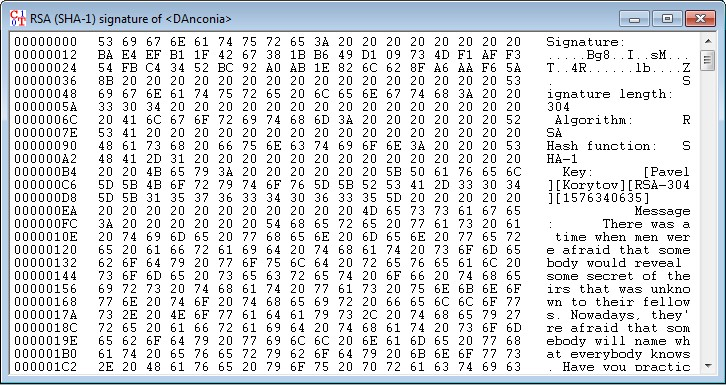
\includegraphics[width=\textwidth]{img/S015.jpg}
            \caption{Подписанное сообщение}%
        \end{figure}
        \FloatBarrier{}
        
    \end{enumerate}
\end{enumerate}

\section{Подписание своего отчёта}
\subsection{Формулировка задания}
\begin{enumerate}
    \item Сконвертируйте отчёт в формат pdf
    \item Экспортируйте ранее созданный сертификат ключевой пары RSA Digital Signatures/PKI->PKI/Generate…->Export PSE (\#PKCS12).
    \item Откройте pdf-версию отчета и попытайтесь подписать с использованием этого сертификата.
    \item Создайте собственный самоподписанный сертификат в среде Adobe Reader и используйте его для подписи отчета.
    \item Сохраните скриншоты свойств подписи и сертификата
    \item Внесите изменения (маркеры, комментарии) в отчёт и проверьте подпись.
\end{enumerate}

\subsection{Ход работы}
\begin{enumerate}
    \item Текущая версия отчёта скомпилирована в pdf.
    \item Созданный сертификат экспортирован в формат p12.
    \item Т.к. на Linux нет Adobe Acrobat, установлена программа Portable Signer. Произведено подписание документа.
    \begin{figure}[h]
        \centering
        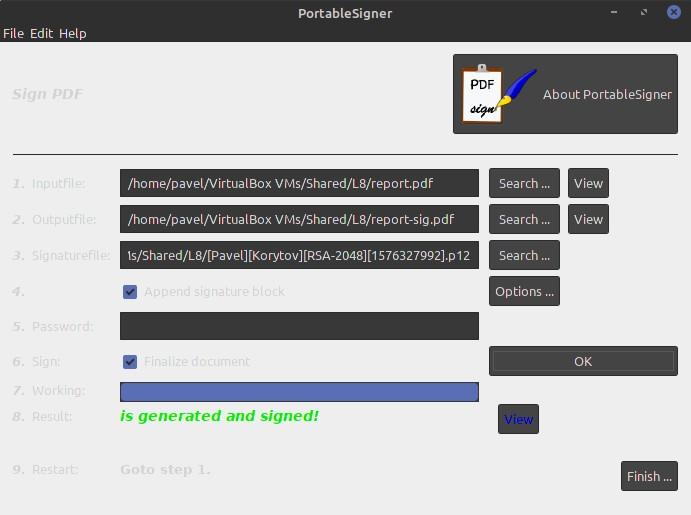
\includegraphics[width=\textwidth]{img/S020.jpg}
        \caption{Интерфейс программы}%
    \end{figure}
    \begin{figure}[h]
        \centering
        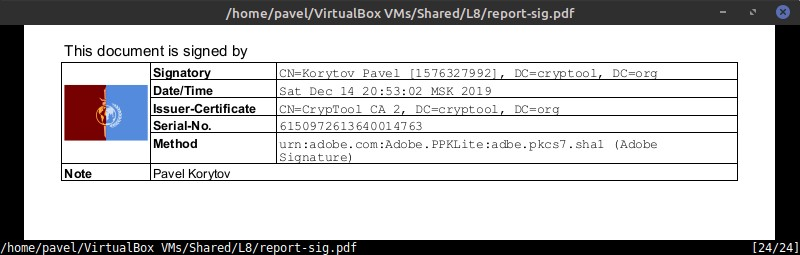
\includegraphics[width=\textwidth]{img/S021.jpg}
        \caption{Знак подписи}%
    \end{figure}
    \item С помощью утилиты pdfsig проведена проверка подписи
    \begin{figure}[h]
        \centering
        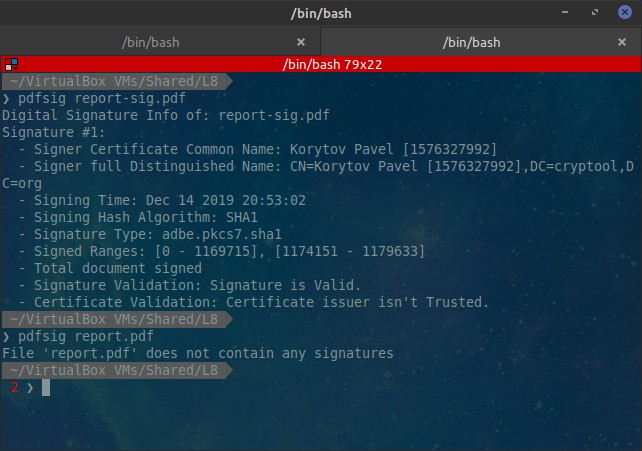
\includegraphics[width=\textwidth]{img/S022.jpg}
        \caption{Проверка подписи}%
    \end{figure}
    \FloatBarrier{}
    Сертификат верен.
    \item Проведена модификация pdf-файла.
    \begin{figure}[h]
        \centering
        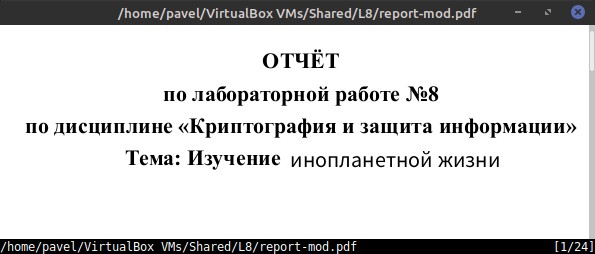
\includegraphics[width=\textwidth]{img/S023.jpg}
        \caption{Модифицированный файл}%
    \end{figure}
    \FloatBarrier{}

    \item Проведена проверка дайджеста
    \begin{figure}[h]
        \centering
        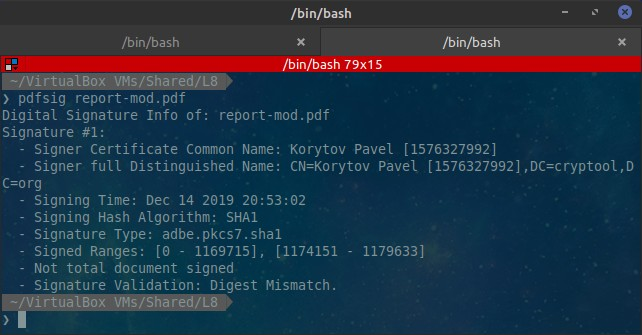
\includegraphics[width=\textwidth]{img/S024.jpg}
        \caption{Проверка подписи модифицированного файла}%
    \end{figure}
    \FloatBarrier{}

    Изменение обнаружено.
    
\end{enumerate}

\clearpage
\section{Выводы}
Исследованы алгоритмы создания и проверки цифровой подписи, алгоритмы генерации ключевых пар RSA, DSA, ECDSA.\@ Изучена работа с ними в CrypTool 1.

Алгоритм RSA основывается на задаче факторизации, DSA --- на задаче дискретного логарифмирования. ECDSA --- модификация DSA, работающая не в кольце целых чисел, но в группе точек эллиптической кривой.

Цифровая подпись --- результат криптографической-хэш функции от документа. Цифровая подпись создается секретно (с помощью закрытого ключа), но может быть публично проверена (с помощью открытого ключа).

Сертификат открытого ключа содержит:
\begin{itemize}
    \item Открытый ключ владельца сертификата
    \item Срок действия
    \item Имя выдающего
    \item Имя владельца сертификата
    \item Цифровой подписи\\
\end{itemize}

Сертификат выдается центром сертификации, открытый ключ центра общеизвестен. Любой, имеющий сертификат, может проверить подлинность сертификата, как следствие --- подлинность открытого ключа владельца. Таким образом, можно проверить подлинность подписи документа.

\end{document}
